\documentclass[twoside, 10pt]{amsart}

% PACKAGES


\usepackage{fullpage}
\usepackage{amscd}
\usepackage{amsmath}
\usepackage{amssymb}
\usepackage{amsthm}
\usepackage{color}
\usepackage{graphicx}
\usepackage{hyperref}
\usepackage[noabbrev,capitalize]{cleveref}
\usepackage{mathrsfs}
\usepackage{mathtools}
\usepackage{pict2e}
\usepackage{stackrel}
\usepackage[T1]{fontenc}
\usepackage{tikz}
\usepackage{tikz-cd}
\usetikzlibrary{decorations.pathmorphing,arrows}
\usepackage[utf8]{inputenc}
\usepackage{wasysym}
\usepackage[all]{xy}
\usepackage{xcolor}
\usepackage{xy}
\usepackage{a4wide}

\hypersetup{
    colorlinks,
    linkcolor={red!50!black},
    citecolor={blue!50!black},
    urlcolor={blue!80!black}
}

\usepackage[lf]{Baskervaldx} % lining figures
\usepackage[bigdelims,vvarbb]{newtxmath} % math italic letters from Nimbus Roman
\usepackage[cal=boondoxo]{mathalfa} % mathcal from STIX, unslanted a bit
\renewcommand*\oldstylenums[1]{\textosf{#1}}

\allowdisplaybreaks

% INDENTATION

\setlength{\parindent}{0pt}

% LEMMAS, THEOREMS, ETC.

\newtheorem{lemma}{Lemma}[section]
\newtheorem{remark}[lemma]{Remark}
\newtheorem{example}[lemma]{Example}
\newtheorem{theorem}[lemma]{Theorem}
\newtheorem{corollary}[lemma]{Corollary}
\newtheorem{definition}[lemma]{Definition}
\newtheorem{proposition}[lemma]{Proposition}
\newtheorem{conjecture}[lemma]{Conjecture}
\newtheorem{notation}[lemma]{Notation}

% MACROS

\newcommand{\daniel}[1]{\textcolor{red}{#1}}
\newcommand{\bruno}[1]{\textcolor{blue}{#1}}

% CATEGORY

\newcommand{\sSe}{\mathsf{sSet}}
\newcommand{\sLialg}{\ensuremath{\mathcal{sL}_\infty\text{-}\,\mathsf{alg}}}
\newcommand{\sLiealg}{\ensuremath{\mathcal{s}\lie\,\text{-}\,\mathsf{alg}}}
\def\cD{\mathrm{\Delta}}

% OPERADS

\newcommand{\sLi}{\ensuremath{\mathcal{sL}_\infty}}
\newcommand{\sLie}{\ensuremath{\mathcal{s}\mathrm{Lie}}}
\newcommand{\com}{\ensuremath{\mathrm{Com}}}
\newcommand{\Cobar}{\ensuremath{\Omega}}
\renewcommand{\Bar}{\ensuremath{\mathrm{B}}}
\newcommand{\lie}{\ensuremath{\mathrm{Lie}}}

% ALGEBRAS

\newcommand{\g}{\ensuremath{\mathfrak{g}}}
\newcommand{\wsLi}{\ensuremath{\widehat{\mathcal{sL}_\infty}}}

% FUNCTORS 

\newcommand{\R}{\ensuremath{\mathrm{R}}}
\renewcommand{\L}{\ensuremath{\mathscr{L}}}
\newcommand{\Li}{\mathfrak{L}_\infty}

% AUTRES 

\newcommand{\antishriek}{\mbox{\footnotesize{\rotatebox[origin=c]{180}{$!$}}}}
\newcommand{\RT}{\mathrm{RT}}
\newcommand{\Sy}{\mathbb{S}}
\renewcommand{\d}{\ensuremath{\mathrm{d}}}
\newcommand{\PP}{\ensuremath{\mathrm{P}}}
\def\Ho#1#2{\Lambda^{#2}_{#1}}
\def\De#1{\mathrm{\Delta}^{#1}}
\newcommand{\NN}{\mathbb{N}}
\newcommand{\RR}{\mathbb{R}}

%%%%%%%%
\newcommand{\CC}{\ensuremath{\mathrm{CC}_\infty}}

%%%%%%%%%%%%  NOT INCORPORED YET %%%%%%%%%%%%%%%%%%%%%

\newcommand{\Lalg}{\ensuremath{\mathscr{L}_\infty\text{-}\mathsf{alg}}}

\newcommand{\F}{\ensuremath{\mathrm{F}}}
\newcommand{\h}{\ensuremath{\mathfrak{h}}}


\newcommand{\C}{\ensuremath{\mathscr{C}}}
\newcommand{\D}{\ensuremath{\mathscr{D}}}
\renewcommand{\P}{\ensuremath{\mathscr{P}}}



\newcommand{\End}{\ensuremath{\mathrm{End}}}
\newcommand{\susp}{\ensuremath{\mathscr{S}}}
\newcommand{\T}{\ensuremath{\mathcal{T}}}
\newcommand{\vdl}{\ensuremath{\mathrm{VdL}}}
\newcommand{\Tw}{\ensuremath{\mathrm{Tw}}}
\newcommand{\Hom}{\ensuremath{\mathrm{Hom}}}
\renewcommand{\S}{\ensuremath{\mathbb{S}}}
\renewcommand{\k}{\ensuremath{\mathbb{K}}}
\newcommand{\id}{\ensuremath{\mathrm{id}}}
\newcommand{\MC}{\ensuremath{\mathrm{MC}}}
\newcommand{\mc}{\ensuremath{\mathfrak{mc}}}
\newcommand{\mcoo}{\ensuremath{\mathfrak{mc}^\infty}}
\newcommand{\dgl}{\ensuremath{\mathsf{dgLie}}}


\newcommand{\ad}{\operatorname{ad}}
\newcommand{\PTt}{\ensuremath{\widetilde{\mathrm{PT}}}}
\newcommand{\PT}{\ensuremath{\mathrm{PT}}}

\makeatletter
\newcommand{\whiteleaf}{\mathord{\mathpalette\nicoud@YESNO\relax}}
\newcommand{\blackleaf}{\mathord{\mathpalette\nicoud@YESNO{\nicoud@path{\fillpath}}}}
\newcommand{\nicoud@YESNO}[2]{%
	\begingroup
	\settoheight{\unitlength}{$#1X$}%
	\begin{picture}(0.7,1)
	\linethickness{\variable@rule{#1}}%
	\roundcap\roundjoin
	\nicoud@path{\strokepath}
	#2
	\Line(0.35,0)(0.35,0.5)
	\end{picture}%
	\endgroup
}
\newcommand{\nicoud@path}[1]{%
	\moveto(0.1,0.5)
	\lineto(0.1,1)\lineto(0.6,1)\lineto(0.6,0.5)
	\closepath
	#1
}
\newcommand{\variable@rule}[1]{%
	\fontdimen8  
	\ifx#1\displaystyle\textfont3\else
	\ifx#1\textstyle\textfont3\else
	\ifx#1\scriptstyle\scriptfont3\else
	\scriptscriptfont3\relax
	\fi\fi\fi
}
\makeatletter



% AUTHOR, ETC.

\author{Daniel Robert-Nicoud and Bruno Vallette}
\date{}
\title{Homotopy Lie theory}
\date{\today}
\address{Laboratoire Analyse, G\'eom\'etrie et Applications, Universit\'e Paris 13, Sorbonne Paris Cit\'e, 99 Avenue Jean Baptiste Cl\'ement, 93430 Villetaneuse, France}
\email{\href{mailto:robert-nicoud@math.univ-paris13.fr}{robert-nicoud@math.univ-paris13.fr}}
\address{Laboratoire Analyse, G\'eom\'etrie et Applications, Universit\'e Paris 13, Sorbonne Paris Cit\'e, 99 Avenue Jean Baptiste Cl\'ement, 93430 Villetaneuse, France}
\email{\href{mailto:vallette@math.univ-paris13.fr}{vallette@math.univ-paris13.fr}}

% CLASSIFICATION/KEYWORDS/THANKS

\subjclass[2010]{}

\keywords{}

\thanks{The first author was supported by grants from R\'egion Ile-de-France, the second author was supported by the Institut Universitaire de France, and both authors were supported by the grant ANR-14-CE25-0008-01 project SAT}

\begin{document}

\maketitle

\setcounter{tocdepth}{1}

\begin{abstract}
\bruno{To be typed at the very end.}
\end{abstract}

\tableofcontents

% CONVENTIONS
\hrule
\begin{itemize}
\item Convention homologique
\item $\sLi$-algebras
\item $\sLialg$ : the category of complete $\sLi$-algebras
\item $\alpha$ Maurer--Cartan element
\item $\R$ : representation functor 
\item $C_\bullet$ : objet simplicial
\item $C^\bullet$ : objet cosimplicial
\item $\sSe$ : category of simplicial sets 
\item font sans serif pour les categories 
\item $\k$ field (char $0$)
\item $\mathrm{C}^\bullet:=C(\De{\bullet})$ cellular chain complex (cosimplicial object)
\item $\mathrm{C}_\bullet:=C(\De{\bullet})^\vee$ (co)cellular chain complex (simplicial object)
\item operad $\com$
\item $\CC$-algebras for $\Cobar \Bar \com$-algebras. 
\item $A^\vee$ : linear dual
\item $\mc_\bullet\coloneqq \Cobar_\pi \, \mathrm{C}^\bullet$ : the \emph{Maurer--Cartan cosimplicial $\sLi$-algebra}
\item $\sLie$ : operad
\item $\MC_\bullet$ : Deligne--Hinich $\infty$-groupoid. 
\item $\gamma_\bullet$ : Getzler $\infty$-groupoid
\item $\RT$ set of rooted trees
\item $\overline{\RT}$ : reduced rooted trees (without $|$)
\item $\Sy$ symmetric group
\item $\T$ free operad
\item $\wsLi(V)$ free complete $\sLi$-algebra 
\item $\tau, |\tau|$ : a rooted tree and its number of vertices 
\item $\d$ differentielle de la $\sLi$-algebra
\item $\mathrm{PT}^{[n]}$ : set of planar rooted trees with internal vertices having at least one input  and such that the total number of vertices and leaves is equal to $n$. 
\item $\Ho{k}{n}$ horns \bruno{toujours pas fan des deux petites barres en bas ... Pas trouve mieux}
\item $\De{n}$ ensemble simpliciaux "principaux"
\item $\NN$ : integers
\item $\RR$ : real numbers 
\item $\cD$ simplex category
\end{itemize}
\hrule



\section*{Introduction}
\bruno{To be typed at the very end.}

%Goals: give explicit formul{\ae} for the notion of homotopy between $\infty$-morphisms of $\L_\infty$-algebras given in \cite[Sect. 3]{Vallette14}.
%
%\medskip
%
%Motivation: people need it, e.g. Camille.


\subsection*{Layout}

\subsection*{Conventions}\leavevmode

\bruno{convention homologique : que des complexes de chaines (differentielles de degrees $-1$); les complexes de "cochaines" sont concentres en degrees de $-n$ a $0$ \\
 corps de base \\ 
 (degree-wise, arity-wise) linear dual $A^\vee$.\\}

We work over a field $\k$ of characteristic $0$. 



\section{Recollections \bruno{[Bruno]}}

The classical Lie theory is made of an equivalence between a category of Lie algebras and a category of groups. The higher analogue is actually a Quillen equivalence between a category of homotopy Lie algebras and a category of $\infty$-groupoid, notions that we recall and make precise in this section. \bruno{a reprendre a la fin}. 


\subsection{Complete shifted homotopy Lie algebras}
In this section, we recall the main features of complete shifted homotopy Lie algebras. 


\begin{definition}[Complete dg module]
A \emph{complete differential graded (dg) module} $(A, d, \mathrm{F})$ is a chain complex, i.e. with homological degree convention $|d|=-1$, equipped with a filtration 
\[A=\F_0 A = \F_1 A \supset \F_2 A \supset \cdots \supset \F_k A \supset F_{k+1}A \supset \cdots\]
made up of dg sub-modules, such that the associated topology is complete. 
\end{definition}

Notice that in the present paper, we restrict ourselves to the case $\F_0 A = \F_1 A$. A morphism of complete dg module is a chain map preserves the respective filtrations. 
Any dg module  $V$ is viewed as a complete dg module endowed with the discrete thus complete filtration $V=\F_0 V = \F_1  V\supset \F_2 V= \F_3 V=  \cdots=0$. 

\begin{definition}[Complete shifted  $\L_\infty$-algebra]
A \emph{complete shifted  $\L_\infty$-algebra structure}, on a complete differential graded module $(A, d, \mathrm{F})$ is a collection 
$(\ell_2, \ell_3, \ldots, )\in \prod_{n\geqslant 2} \hom\big(A^{\odot n}, A\big)$ of symmetric maps which respect the filtration, of degree $-1$, and  satisfying 
\[
 \partial\left(\ell_n\right)+\sum_{p+q=n+1\atop 2\leqslant p,q \leqslant n}
\sum_{\sigma\in \mathrm{Sh}_{p,q}^{-1}}
 (\ell_{p+1}\circ_{1} l_q)^{\sigma}=0\ ,
\]
where $ \mathrm{Sh}_{p,q}^{-1}$ denotes the set of the inverses of $(p,q)$-shuffles.
\end{definition}

These are actually algebras over the operad $\sLi:=\susp\otimes \L_\infty\cong \Cobar \com^\vee$, which is the suspension of the operad encoding $\L_\infty$-algebra. So we will call them \emph{complete $\sLi$-algebras}. 
In the present paper, we  consider the category of algebras over this operad, denoted $\sLialg$, that is with 
 strict morphisms of $\sLi$-algebras, which are made up of one map of degree $0$ commuting strictly with the structure operations. This operadic interpretation over the symmetric monoidal category of complete dg modules with the completed tensor product $\widehat{\otimes}$ \cite{DotsenkoShadrinVallette18} allows us to apply to complete $\sLi$-algebras all the classical operadic constructions and results \cite{LodayVallette12}, like the following one.
 
 \begin{proposition}\label{prop:CatCocomp}
 The category of complete $\sLi$-algebras is locally small, complete, and cocomplete. 
 \end{proposition}
 
\begin{proof}
All the arguments of  \cite[Lemma~4]{DotsenkoShadrinVallette18} hold true for complete dg modules whose filtration satifises $\F_0=\F_1$. Therefore this latter category is locally small, complete, and cocomplete and thus is the category of complete $\sLi$-algebras as a category of algebras over an operad, by \cite[Theorem~1]{DotsenkoShadrinVallette18}.
\end{proof}
 
\begin{remark} 
By definition of  the suspension operad $\susp:=\End_{\k s}$, the category of (complete)  $\sLi$-algebras is isomorphic to the category of $\L_\infty$-algebras, the two isomorphism functors are given by the (de)suspension of the underlying chain complexes: $\g \mapsto s^{\pm 1}\g$. In the present context, $\sLi$-algebras appear more naturally than their analogues and they have the great advantage of carrying much less signs (if not none).
\end{remark}

\begin{definition}[Maurer--Cartan element]
A \emph{Maurer--Cartan element} is a degree $0$ element $\alpha\in \g_0$ of a complete $\sLi$-algebras satifying the Maurer--Cartan equation:
\[
d(\alpha)+\sum_{n\geqslant 2} {\textstyle \frac{1}{n!}}\ell_n(\alpha, \ldots, \alpha)=0 \ ;
\]
the associated set is denoted by $\MC(\g)$.
\end{definition}

For any $n\geqslant 2$, we consider the set $\RT_n$ of rooted trees with $n$ leaves such that each vertex as at least two inputs. The set $\RT_1:=\{|\}$ is made up of the trivial rooted tree. We denote the number of vertices of a rooted tree $\tau\in\RT$ by $|\tau|$. The set of \emph{reduced} rooted trees, that is without the trivial tree, is denoted by $\overline{\RT}$. 

%The homological degree of any vertex is equal to $-1$; so the degree $|\tau|$ of a rooted tree $\tau\in \RT$ is equal to  minus this number of vertices.

\begin{proposition}
Let $V$ be a dg module with basis $\{v_i\}_{i\in I}$. The free complete $\sLi$-algebra generated by $V$ is isomorphic to the following product
\[\wsLi(V):=\sLi\, \widehat{\circ}\,  V\cong \prod_{n\geqslant 1}
\sLi(n)\otimes_{\Sy_n} V ^{\otimes n}  \ ,\]
with a basis given series indexed by  $n$ of linear combinations of rooted trees $\tau$, of degree $-|\tau|$, with $n$ leaves labelled by elements $v_i$. 
\[\vcenter{\hbox{
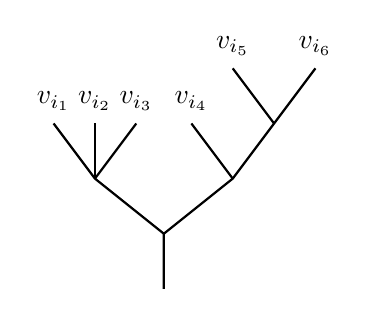
\begin{tikzpicture}[yscale=0.7,xscale=0.7]

\draw[thick] (-2,2)--(-1.25,1) -- (0,0) -- (0,-1);
\draw[thick] (-1.25,2) -- (-1.25,1); 
\draw[thick] (-0.5,2) -- (-1.25,1); 
\draw[thick] (0,0) -- (1.25,1) -- (2,2)--(2.75,3); 
\draw[thick] (0.5,2) -- (1.25,1); 
\draw[thick] (1.25,3) -- (2,2); 


\node at (-2,2.4) {$v_{i_1}$};
\node at (-1.25,2.4) {$v_{i_2}$};
\node at (-0.5,2.4) {$v_{i_3}$};
\node at (0.5,2.4) {$v_{i_4}$};
\node at (1.25,3.4) {$v_{i_5}$};
\node at (2.75,3.4) {$v_{i_6}$};
\end{tikzpicture}}}\]
The differential is the sum of the internal differential on $V$ with the splitting of all corollas into two. 
The operations $\ell_n$ amounts to graft $n$ rooted trees to $n$ leaves of a corolla.
\end{proposition}

\begin{proof}
The set $\RT$ of rooted trees provides us with a basis of the operad $\sLi\cong\Cobar \com^\vee\cong \T\big(s^{-1} \overline{\com}\big)$. The form of the complete free algebra on a discrete dg module follows from \cite[Section~2.2]{DotsenkoShadrinVallette18}. The differential and the structure operations are produced by the general theory of operads, see \cite[Section~6.5.2]{LodayVallette12}. 
\end{proof}

\subsection{Algebraic $\infty$-groupoid}



\begin{definition}[Simplex category $\cD$]
The \emph{simplex category}, denoted by $\cD$, has, for objects, the totally ordered sets 
 $[n]=\{0<  \cdots< n\}$, for  $n\in \NN$, and, for morphisms, the order-preserving maps. 
\end{definition}

\begin{definition}[Simplicial set]
The category of \emph{simplicial sets}, denoted by $\sSe$, is the category of presheaves 
$\sSe:=\mathsf{Fun(}\cD^\mathsf{op}, \mathsf{Set)}$
over the simplex category. 
\end{definition}

Presheaves over the opposite category are called \emph{cosimplicial sets}. To avoid confusion, when it is necessary, we denote simplicial sets by $X_\bullet$ and respectively cosimplicial sets by $X^\bullet$. 

\begin{example}
For $n\in \NN$, the \emph{standard $n$-simplex} is the simplicial set 
$\De{n}:=\Hom_{\cD}(-,[n])$ represented by $[n]$. This combinatorial object encodes the cellular decomposition of the \emph{geometric $n$-simplex}, which is the convex hull of the unit vectors in $\RR^{n+1}$:
\[|\De{n}|:=\left\{
(t_0, \ldots, t_n) \in [0,1]^{n+1}\, | \, t_0+\cdots+t_n=1
\right\} \ .\]
\end{example}

\begin{definition}[Horn]
The \emph{$k^{\text{th}}$ horn $\Ho{k}{n}$ of dimension $n$}, for $n\geqslant 2$ and $0\leqslant k \leqslant n$, is 
\bruno{...}
\end{definition}

We call an \emph{$n$-horn} in a simplicial set $X_\bullet$ a morphism of simplicial sets 
$\Ho{k}{n}\to X_\bullet$ and a \emph{horn filler} a morphism of simplicial sets $\De{n}\to X_\bullet$ which lifts the horn:
\[
\vcenter{\hbox{
\begin{tikzcd}[column sep=0.8cm, row sep=1cm]
\Ho{k}{n}
\arrow[d, hookrightarrow]
\arrow[r]
& X_\bullet
\\
\De{n} \arrow[ur, dashrightarrow] 
&\end{tikzcd}
}}\ .
\]

\begin{definition}[Kan complex]
A \emph{Kan complex} is simplicial set $X_\bullet$ for which every horn $\Ho{k}{n}\to X_\bullet$, for $n\geqslant 2$ and $0\leqslant k \leqslant n$, can be filled.
\end{definition}

\begin{proposition}[{see \cite[Lemma~3.3]{GoerssJardine09}}]
The singular simplicial set $\Hom_{\mathsf{Top}}(|\De{\bullet}|, X)$ associated to any topological space $X$ is a Kan complex.
\end{proposition}
 Moreover, the singular simplicial set functor is faithful (but not full) and Kan complexes are known to share the same homotopy theory than compactly generated Hausdorff spaces notably after the seminal works of D. Quillen \cite{Quillen67}. 
That is why, many people refer to Kan complexes simply as to ``spaces''. 

The notion of a Kan complex is a property, one can get make it into a structure by the following definition due to T. Nickolaus in \cite{Nickolaus11}, called algebraic Kan complex in \textit{loc. cit.}. 

\begin{definition}[Algebraic $\infty$-groupoid]
An \emph{algebraic $\infty$-groupoid} is a simplicial set $X_\bullet$ with a given filler for which every horn $\Ho{k}{n}\to X_\bullet$, for $n\geqslant 2$ and $0\leqslant k \leqslant n$.
\end{definition}

\begin{proposition}
The nerve of a groupoid but here we have no choice: there exists one and only one horn filler each time. 
\end{proposition}

\bruno{A reprendre ! 
modeles pour les $\infty$-groupoid, hypothese homotopique, notion de complexe de Kan algebrique de Nickolaus ("mieux que Getzer"). Terminologie : "Algebraic $\infty$-groupoid" (ou "algebraic Kan complex") car structure algebrique, pas propriete?}

We refer the reader to \cite{GoerssJardine09} for more details on simplicial sets and their homotopy properties. 
\section{Cosimplicial object \bruno{[Bruno]}}

\subsection{Dold--Kan correspondence}

Let us start with the following observation, which  goes back to D.M. Kan. 

\begin{lemma}[{\cite{Kan58bis}}]\label{lem:AdjCosimpliObj}
Let $\mathsf{C}$ be a locally small cocomplete category. 
The data of a pair of adjoint functors whose left adjoint has domain in simplicial sets 
\[ 
\vcenter{\hbox{
\begin{tikzcd}
{\ \ \mathrm{L} \ : \ \sSe}
\arrow[r, harpoon, shift left=0.9ex, "\perp"']
&
\arrow[l, harpoon,  shift left=0.9ex]
\mathsf{C}\ : \ \mathrm{R}\ 
\end{tikzcd}
}}
\]
is equivalent to the data of a cosimplicial objects
$\mathrm{C}^\bullet : \De{} \to \mathsf{C}$
 in $\mathsf{C}$, under the restriction 
\[
\vcenter{\hbox{
\begin{tikzcd}
\mathrm{C}^\bullet=\mathrm{L}\mathrm{Y}\ : \ \cD
\arrow[r, "\mathrm{Y}"]
&
\sSe \arrow[r, "\mathrm{L}"]
&
\mathsf{C}
\end{tikzcd}
}}
\]
of the left adjoint functor to  the Yoneda embedding $\mathrm{Y}$. 
\end{lemma}

\begin{proof}
Any cosimplicial object $\mathrm{C}^\bullet : \cD \to \mathsf{C}$ induces a functor 
\[
\begin{array}{ccrcl}
\mathrm{R} &:&\mathsf{C} & \to & \sSe
\\
&&c &\mapsto& \Hom_{\mathsf{C}}(\mathrm{C}^\bullet, c)\ , 
\end{array}
\]
which admits a left adjoint given by the following left Kan extension: 
\[\vcenter{\hbox{\begin{tikzcd}
\cD \arrow[rr, "\mathrm{C}^\bullet"] \arrow[hookrightarrow, dr, "\mathrm{Y}"']&  
& \mathsf{C} \\
&\sSe \arrow[ur, "\mathrm{Lan}_\mathrm{Y} \mathrm{C}^\bullet"']&
\end{tikzcd}}}\ .\]
Finally, notice that left adjoint functors preserve colimits and that there is a unique  colimit preserving functor $\mathrm{L} : \sSe \to \mathsf{C}$ with prescribed restriction to $\cD$, by the density theorem: any simplicial set $X_\bullet$ is isomorphic to the colimit 
$$X_\bullet\cong \mathop{\rm colim}_{\mathsf{E}(X_\bullet)} \mathrm{Y}\circ \Pi \ .$$
over its category of elements, where 
  $\Pi : \mathsf{E}(X_\bullet) \to \cD$ is the canonical projection which sends $x\in X_n$ onto $[n]$. 
\end{proof}

This fact shows that if one wants to introduce a functor from a category $\mathsf{C}$ to simplicial sets, a good way is to consider a cosimplicial objects in $\mathsf{C}$. 

\begin{example}
Let $\mathsf{C}=\mathsf{dg Mod}$ be the category of dg modules. We consider the cosimplicial dg module 
\[\mathrm{C}^\bullet:=C(\De{\bullet})\]
made up of the cellular chain complexes of the geometric $n$-simplicies $|\De{n}|$ or equivalently the normalised chain complex of the standard $n$-simplicies $\De{n}$. The associated adjonction 
\[
\vcenter{\hbox{
\begin{tikzcd}
{\ \ \mathrm{L}_{\mathrm{DK}} \ : \ \sSe}
\arrow[r, harpoon, shift left=0.9ex, "\perp"']
&
\arrow[l, harpoon,  shift left=0.9ex]
\mathsf{dg Mod}\ : \ \mathrm{R}_{\mathrm{DK}}\ 
\end{tikzcd}
}}
\]
is nothing but the one involved in the Dold--Kan correspondence: equivalence of categories between abelian simplicial abelian groups and non-negatively graded chain complexes of abelian groups.
\end{example}

\bruno{mettre aussi l'exemple du foncteur singulier et de la realisation geometrique ? Coupe le flot mais on s'en sert (un peu) dans la partie categorie de modeles}

\subsection{Maurer--Cartan cosimplicial complete $\sLi$-algebra}

In the present paper, we work with the  category $\mathsf{C}=\sLialg$ of complete $\sLi$-algebras. To define in this category a suitable cosimplicial object, we consider the following elements involved in Dupont's simplicial version of  the de Rham Theorem. 

\begin{proposition}[{\cite{Dupont76}}]
There exists a simplicial contraction 
\begin{center}
	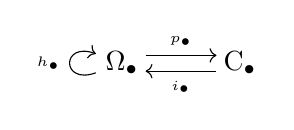
\begin{tikzpicture}
	\node (a) at (0,0){$\Omega_\bullet$};
	\node (b) at (1.5,0){$\mathrm{C}_\bullet$};
	
	\draw[->] (a)++(.3,.1)--node[above]{\mbox{\tiny{$p_\bullet$}}}+(0.9,0);
	\draw[<-,yshift=-1mm] (a)++(.3,-.1)--node[below]{\mbox{\tiny{$i_\bullet$}}}+(0.9,0);
	\draw[->] (a) to [out=-160,in=160,looseness=5] node[left]{\mbox{\tiny{$h_\bullet$}}} (a);
	\end{tikzpicture}
\end{center}
between the simplicial dg commutative algebras of piecewise polynomial differential forms on the geometric $n$-simplicies 
\[
\Omega_n:=\k[t_0, \ldots, t_n, d t_0, \ldots, d t_n]/(t_0+\cdots+t_n-1, d t_0+\cdots+ d t_n)
\]
and the simplicial dg module made up of the linear dual of the cellular chain complexes of the geometric $n$-simplicies 
\[\mathrm{C}_\bullet:=C(\De{\bullet})^\vee\ .\]
\end{proposition}

\begin{remark}
Since we work with the homological degree convention, the elements $d t_i$ have all degree $-1$ and the dg module $C(\De{n})^\vee$ is concentrated in degree range $-n$ to $0$ with differential of degree $-1$. 
% In order to view these two chain complexes in the category of complete dg modules, we endow both of them with the discrete filtration: 
%$\F_0  = \F_1  \supset \F_2 = \F_3= \cdots=0$ \ .
\end{remark}

The former chain complex carries an algebra structure over the operad $\com$, which admits a canonical cofibrant replacement by means of the bar-cobar construction $\Cobar \Bar \com \xrightarrow{\sim} \com$. By pulling back, each $\Omega_n$ carries an $\Cobar \Bar \com$-algebra structure that we can transfer onto 
$C(\De{n})^\vee$ under the homotopy transfer theorem, see \cite[Section~10.3]{LodayVallette12} for instance.
Since the Dupont contraction is simplicial, the various maps can be extended to $\infty$-morphisms in order to form a simplicial $\Cobar \Bar \com$-algebra structure on $C(\De{\bullet})^\vee$. 
Since the $C(\De{n})^\vee$ are degree-wise finite dimensional  and since $\Cobar \Bar \com$ is degree-wise and arity-wise finite dimensional, the cellular chain complexes $\mathrm{C}^\bullet=C(\De{\bullet})$ admit a cosimplicial $\Bar \Cobar \com^\vee\cong \left(
\Cobar \Bar \com\right)^\vee$-coalgebra structure. 
The canonical twisting morphism $\pi \colon \Bar \Cobar \com^\vee \to \Cobar \com^\vee\cong \sLi$ induces a bar-cobar adjonction between complete $\sLi$-algebras and $\Bar \Cobar \com^\vee$-coalgebras, see \cite[Section~11.2]{LodayVallette12}: 
\[
\vcenter{\hbox{
\begin{tikzcd}
{\Cobar_\pi \ : \ \Bar \Cobar \com^\vee\text{-}\,\mathsf{coalg}}
\arrow[r, harpoon, shift left=0.9ex, "\perp"']
&
\arrow[l, harpoon,  shift left=0.9ex]
\sLialg \ : \ \Bar_\pi\ .
\end{tikzcd}
}}
\]

\begin{proposition}\label{prop:Simpli}
All together, the $\Cobar_\pi \mathrm{C}^\bullet$ form a cosimplicial complete $\sLi$-algebra. 
\end{proposition}

\begin{proof}
It remains to notice that the cobar functor $\Cobar_\pi$ sends $\infty$-morphisms of $\Bar \Cobar \com^\vee$-coalgebras to strict morphisms of $\sLi$-algebras, see  \cite[Section~3]{rnw17}.
\end{proof}


\begin{definition}[The Maurer--Cartan cosimplicial $\sLi$-algebra]
The \emph{Maurer--Cartan cosimplicial $\sLi$-algebra} is defined by 
\[
\mc_\bullet\coloneqq \Cobar_\pi \mathrm{C}^\bullet\ .
\]
\end{definition}

Let us now try to make this seminal object more explicit. The proof of the following fact will give more details. 

\begin{proposition}\label{prop:mc0}
The $0$-simplex $\mc_0$ is the free complete $\sLi$-algebra on one Maurer--Cartan element:
\[\mc_0\cong 
\big(\widehat{\sLi}(a_0), \d(a_0)=-\sum_{m\geqslant 2} {\textstyle \frac{1}{m!}}\ell_m(a_0, \ldots, a_0)
\big)
\ .\]
\end{proposition}

\begin{proof}
The chain complex $C(\De{n})^\vee$ can be seen as a sub-chain complex of $\Omega_n$ spanned by the  basis made up of the differential forms  $\omega_I$, for $I=\{i_0,\ldots, i_k\}\subset[n]$, with degree $|\omega_I|=-|I|=-k-1$:
\[
\omega_{i_0\cdots i_k}:=k!\sum_{j=0}^k (-1)^jt_{i_j} dt_{i_0}\cdots \widehat{dt_{i_j}}\cdots dt_{i_k} \ .
\]
For $n=0$, the dg commutative algebra $\Omega_0=\k \omega_0={\k} 1$ is trivial and the chain complex 
$C(\De{n})^\vee=\k \omega_0$ is one-dimensional. 

Since the dg operad $\Cobar \Bar \com$ is quasi-free on $s^{-1} \Bar \com=s^{-1}\T^c\big(s\overline{\com}\big)$, the transferred $\Cobar \Bar \com$-algebra structure on $C(\De{n})^\vee$ amounts to a collection of operations 
$\{\mu_\tau\}_{\tau \in \RT}$ indexed by rooted trees. The operation $\mu_{|}=\id$ is the identity. Given a rooted tree $\tau\in \RT_m$, the associated operation $\mu_\tau : \left(C(\De{n})^\vee\right)^{\otimes m} \to C(\De{n})^\vee$ has degree $|\tau|-1$ and is explicitly given by the formula 
\[\mu_\tau\left(
\omega_{I_1}, \ldots, \omega_{I_6}
\right)=
\vcenter{\hbox{
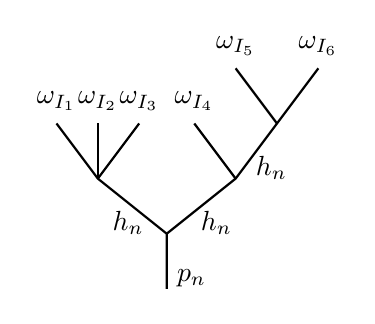
\begin{tikzpicture}[yscale=0.7,xscale=0.7]

\draw[thick] (-2,2)--(-1.25,1) -- (0,0) -- (0,-1);
\draw[thick] (-1.25,2) -- (-1.25,1); 
\draw[thick] (-0.5,2) -- (-1.25,1); 
\draw[thick] (0,0) -- (1.25,1) -- (2,2)--(2.75,3); 
\draw[thick] (0.5,2) -- (1.25,1); 
\draw[thick] (1.25,3) -- (2,2); 

\node at (-2,2.4) {$\omega_{I_1}$};
\node at (-1.25,2.4) {$\omega_{I_2}$};
\node at (-0.5,2.4) {$\omega_{I_3}$};
\node at (0.5,2.4) {$\omega_{I_4}$};
\node at (1.25,3.4) {$\omega_{I_5}$};
\node at (2.75,3.4) {$\omega_{I_6}$};

\node at (-0.7,0.2) {$h_n$};
\node at (0.9,0.2) {$h_n$};
\node at (1.9,1.2) {$h_n$};
\node at (0.45,-0.8) {$p_n$};
\end{tikzpicture}}},\]
where the corollas means the (iterated) commutative product in $\Omega_n$.

For $n=0$, the contracting homotopy $h_0=0$ vanishes and only the operations indexed by corollas $c_m$ do not collapse:
$\mu_{c_m}(\omega_0, \ldots, \omega_0)=\omega_0$\ . 

Let us denote by $a_I:=\omega_I^\vee$ the dual basis on $C(\De{n})$. The linear dual of the operad algebra structure corresponding to $s^{-1} \Bar \com\left(C(\De{n})^\vee \right)\to C(\De{n})^\vee$ produces the cooperad algebra structure corresponding to $C(\De{n})\to s \Cobar \com^\vee\left(C(\De{n})\right)$\ . Notice that, since this linear dual includes the isomorphism between invariants and coinvariants under the actions of the symmetric groups $\Sy_m$, it carries a coefficient ${\textstyle \frac{1}{m!}}$. So, if the element $\lambda \omega_J$, with $\lambda \in \k$, appears in  a product $\mu_\tau\left(
\omega_{I_1}, \ldots, \omega_{I_m}\right)$, then, dually, the image under 
the coproduct map of the element $a_J$ includes the term ${\textstyle \frac{1}{\lambda.m!}} s\tau(  
a_{I_1}, \ldots, a_{I_m})$. 

For $n=0$, the image under the coproduct map of $a_0$ is equal to 
\[
a_0\mapsto \sum_{m\geqslant 1} {\textstyle \frac{1}{m!}} s c_m(a_0, \ldots, a_0)\ .
\]

The cobar construction $\Omega_\pi C(\De{n})$ admits the free complete $\sLi$-algebra on $C(\De{n})$
\[\widehat{\sLi}\big(C(\De{n})\big)\cong 
\widehat{\sLi}\big(a_I,\, I\subset[n]\big)
\]
 as underlying module; its differential is produced by the 
 difference between the internal differential of the chain complex $C(\De{n})$ and the 
 desuspension of the above coalgebra structure, without the primitive term, that is:
\[\d(a_J)= 
\sum_{l=0}^{k} (-1)^{l} a_{j_0\ldots \widehat{j_l} \ldots j_k}
-\sum_{\tau \in \overline{\RT}} {\textstyle\frac{1}{\lambda.6!}}\!\!\!
\vcenter{\hbox{
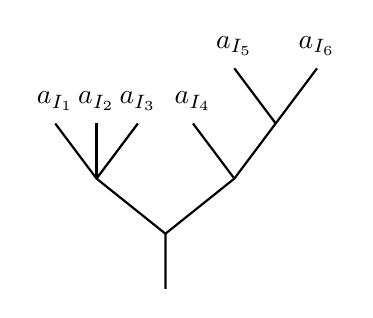
\begin{tikzpicture}[yscale=0.7,xscale=0.7]

\draw[thick] (-2,2)--(-1.25,1) -- (0,0) -- (0,-1);
\draw[thick] (-1.25,2) -- (-1.25,1); 
\draw[thick] (-0.5,2) -- (-1.25,1); 
\draw[thick] (0,0) -- (1.25,1) -- (2,2)--(2.75,3); 
\draw[thick] (0.5,2) -- (1.25,1); 
\draw[thick] (1.25,3) -- (2,2); 

\node at (-2,2.4) {$a_{I_1}$};
\node at (-1.25,2.4) {$a_{I_2}$};
\node at (-0.5,2.4) {$a_{I_3}$};
\node at (0.5,2.4) {$a_{I_4}$};
\node at (1.25,3.4) {$a_{I_5}$};
\node at (2.75,3.4) {$a_{I_6}$};
\end{tikzpicture}}}\ ,\ 
\text{for} \ J=\{j_0, \ldots, j_k\}\ .
\]
For $n=0$, this 
\[\d(a_0)=-\sum_{m\geqslant 2} {\textstyle \frac{1}{m!}}\ell_m(a_0, \ldots, a_0)\ ,\]
which concludes the proof. 
\end{proof}

%\begin{definition}[$\CC$-algebras]
%An algebra over the operad $\Cobar \Bar \com$ is called a \emph{$\CC$-algebras}. Such a structure amounts to a chain complex $(A, d)$ equipped with a collection of operations $\mu_\tau \colon A^{\otimes n} \to A$ indexed by the set of rooted trees with internal vertices having at least two inputs. The arity of the operation $\mu_\tau$ is the number of leaves of the tree $\tau$ and its degree is equal to the number of the vertices of $\tau$ minus $1$. 
%\end{definition}
%
%\bruno{relations ?}

\subsection{Non-abelian Dold--Kan adjunction}
The Maurer--Cartan cosimplicial $\sLi$-algebra 
$\mc_\bullet$ induces canonically the following pair of adjoint functors. 

\begin{definition}[Simplicial representation]\label{def:SimpRep}
The \emph{simplicial representation of complete $\sLi$-algebras}  is produced by the  functor 
\[
\begin{array}{ccrcl}
\mathrm{R} &:&\sLialg & \longrightarrow & \sSe
\\
&&\g &\longmapsto& \Hom_{\,\sLialg}\left(\mc_\bullet, \g\right) \ .
\end{array}
\]
\end{definition}

As a direct corollary of  Proposition~\ref{prop:mc0}, we have
\[
\R(\g)_0=\Hom_{\,\sLialg}\left(\mc_0, \g\right)\cong \MC(\g)\ .
\]

\begin{definition}[Realisation functor]
The \emph{$\sLi$-realisation functor} is defined by 
\[\Li\coloneqq \mathrm{Lan}_\mathrm{Y} \mc_\bullet\ : \ \sSe \to \sLialg \ .
\] 
\end{definition}

\begin{theorem}\label{thm:MainAdjunction}
The simplicial representation functor is right adjoint to the $\sLi$-realisation functor: 
\[
\vcenter{\hbox{
\begin{tikzcd}
{\Li \ : \ \sSe}
\arrow[r, harpoon, shift left=0.9ex, "\perp"']
&
\arrow[l, harpoon,  shift left=0.9ex]
\sLialg\ : \ \mathrm{R}\ .
\end{tikzcd}
}}
\]
\end{theorem}

\begin{proof}
This is a direct corollary of Lemma~\ref{lem:AdjCosimpliObj} and Proposition~\ref{prop:Simpli}. 
\end{proof}

The sub-category of (complete) abelian $\sLi$-algebras, where all the operations $\ell_n$, i.e. for $n\geqslant 2$, are trivial, is nothing but the category of (complete) dg modules. 

\begin{proposition}
The two simplicial sets which are obtained from a complete dg module under the Dold--Kan representation functor and the $\sLi$-representation functor are isomorphic. 
\end{proposition}

\begin{proof}
Let $\g$ be a complete dg module, viewed as a complete abelian $\sLi$-algebra. Its image under the $\sLi$-representation functor is equal to 
\begin{eqnarray*}
\R(\g)=\Hom_{\,\sLialg}\left(\mc_\bullet, \g\right)=\Hom_{\,\sLialg}\left(\wsLi\left(\mathrm{C}^\bullet\right), \g\right)\cong
\Hom_{\mathsf{dg Mod}}\left(\mathrm{C}^\bullet, \g\right)=\R_{\mathrm{DK}}(\g)\ .
\end{eqnarray*}
\end{proof}

The sub-category of (complete)  $\sLi$-algebras where all the operations $\ell_n$ are trivial, for $n\geqslant 3$, is nothing but the category of (complete) shifted dg Lie algebras. This latter category is controlled by the operad 
$\sLie:=\susp\otimes \lie$. In the same way as above, one can consider the cofibrant Koszul resolution 
$\Cobar  \com^{\antishriek} \xrightarrow{\sim} \com$, and then endow  $C(\De{\bullet})^\vee$ with a simplicial $\Cobar  \com^{\antishriek}$-algebra structures by the homotopy transfer theorem. Its linear dual $C(\De{\bullet})$ thus admits a cosimplicial 
$\Bar\,  \sLie\cong \big(
\Cobar  \com^{\antishriek}\big)^\vee$-coalgebra structure. Finally, the bar-cobar adjunction associated to the 
canonical twisting morphism $\bar{\pi} \colon\Bar\,  \sLie \to  \sLie$, 
\[
\vcenter{\hbox{
\begin{tikzcd}
{\Cobar_{\bar{\pi}} \ : \ \Bar\,  \sLie\,\text{-}\,\mathsf{coalg}}
\arrow[r, harpoon, shift left=0.9ex, "\perp"']
&
\arrow[l, harpoon,  shift left=0.9ex]
\sLiealg \ : \ \Bar_{\bar{\pi}}\ ,
\end{tikzcd}
}}
\]
produces the following cosimplicial complete dg Lie algebra:
\[
\overline{\mc}_\bullet\coloneqq \Cobar_{\bar{\pi}} \,  \mathrm{C}^\bullet\ .
\]
The associated pair of adjoint functors 
\[
\vcenter{\hbox{
\begin{tikzcd}
{\mathfrak{L} \ : \ \sSe}
\arrow[r, harpoon, shift left=0.9ex, "\perp"']
&
\arrow[l, harpoon,  shift left=0.9ex]
\sLiealg\ : \ \overline{\mathrm{R}}
\end{tikzcd}
}}
\]
is the one introduced in \cite{BFMT16}, but in another way. To see this, one just has to prove that  \bruno{XXX}. 

\begin{proposition}
The two simplicial sets which are obtained from a complete dg Lie algebra respectively  under the $\sLie$ and the $\sLi$-representation functors are isomorphic. 
\end{proposition}

\begin{proof}
\bruno{to be finished}

\end{proof}

To sum up, the present $\sLi$-representation functor extends both the Dold--Kan functor and the $\sLie$-representation functor of Buijs--Felix-Murillo--Tanr\'e. 
\[
\vcenter{\hbox{
\begin{tikzcd}[column sep=1cm, row sep=0.7cm]
& \sLialg\arrow[dl]\\
\sSe& \sLiealg\arrow[l]\arrow[u, hookrightarrow]\\
&\mathsf{dg Mod}\arrow[lu]\arrow[u, hookrightarrow]
\end{tikzcd}
}}
\]

%\Lambda^n_k 
%\arrow[d, hookrightarrow, "\sim"']
%\arrow[r]
%& \R(\g)
%\\
%\Delta^n \arrow[ur, dashrightarrow] 
%&


\section{Relation with Maurer--Cartan spaces \daniel{[Daniel]}}

\subsection{Statement}
The literature has already seen several another ways to define Maurer--Cartan spaces, that is actually Kan complexes, out of a complete $\sLi$-algebra $\g$. One can first consider the \emph{Deligne--Hinich space} \cite{Hinich97bis} made up of the solutions to the Maurer--Cartan equation of the complete $\sLi$-algebra structure on the tensor product with the simplicial dg commutative algebra $\Omega_\bullet$:
\[\MC_\bullet(\g):=\MC\left(\g \, \widehat{\otimes}\, \Omega_\bullet\right)\ .\]
On can then use the Dupont simplicial contraction to transfer this $\sLi$-algebra structure onto $\g\,\widehat{\otimes} \,C_\bullet$ and thus consider $\MC\left(\g\, \widehat{\otimes}\, C_\bullet\right)$ \bruno{references ? RN et Bandiera?}. Finally, one can also consider the \emph{Getzler space} \cite{Getzler09} made up of the kernels of the Dupont's homotopy:
\[\gamma_\bullet(\g):=\left\{
\alpha \in \MC_\bullet(\g)\ | \ 
\big(\id_\g\,\widehat{\otimes}\,h_\bullet\big)(\alpha)=0
\right\}\ .\]

\begin{theorem}\label{thm:MainIsos}
Let $\g$ be a complete $\sLi$-algebra. The various Maurer--Cartan spaces associated to $\g$ are related by the following weak equivalences and isomorphisms:
\[\MC_\bullet(\g) \simeq  \gamma_\bullet(\g)  \cong \MC(\g\,\widehat{\otimes}\, C_\bullet)  \cong \R(\g)\ .
\]
\end{theorem}
E. Getzler first proved the weak equivalence in \cite{Getzler09}. Then, R. Bandiera established the first isomorphism in his Ph.D. thesis \cite{Bandiera14}. Finally, the first named author proved directly the weak equivalence $\MC_\bullet(\g) \simeq \MC(\g\,\widehat{\otimes}\, C_\bullet)$ in \cite{rn17cosimplicial}. What remains to show here is the isomorphism with the present representation functor $\R(\g)$. 

\subsection{XXX}

\subsection{YYY}

\subsection{ZZZ}

\section{Higher Lawrence--Sullivan algebra \daniel{[Daniel]} \bruno{[Bruno]}}

\subsection{Generalisation of the Lawrence--Sullivan algebra to the $\sLi$-case \daniel{[Daniel]}}

\bruno{->Daniel : explain the method, different from Proposition~\ref{prop:mc0}. Describe $\mc_0$ and $\mc_1$. Recover Lawrence--Sullivan Lie algebra from that. }


\subsection{Homotopies between \texorpdfstring{$\infty$}{infinity}-morphisms \bruno{[Bruno]}}
\bruno{I will do it later, when you will have typed the section above}

\section{How to fill horns in Maurer--Cartan spaces\bruno{[Bruno]}}

The image of a topological space under the singular  functor produces a Kan complex, that is a simplicial set whose horns can be filled. The issue is actually how to fill these horns. \bruno{A reprendre}


\subsection{Filling horns \bruno{[Bruno]}}

The following result is the key ingredient of this section. 

\begin{lemma}\label{lemm:Fundamental}
For $n\geqslant 2$, there is an isomorphism of complete $\sLi$-algebras 
\[
\mc_n=\Li\big(\De{n}\big)\cong \Li\big(\Ho{k}{n}\big)\,\widehat{\sqcup}\, \sLi(u, du)\ ,
\]
where $u$ is a generator of degree $n$ and where the differential on the right-hand side is given by $d(u)=du$.
\end{lemma}

\begin{proof}
We consider the following morphism of complete $\sLi$-algebras:
\[
\begin{array}{rcl}
\Li\big(\Ho{k}{n}\big)\,\widehat{\sqcup}\, \sLi(u, du)&  \xrightarrow{\varphi}&\Li\big(\De{n}\big)\\
a_I&\mapsto& a_I\\
u&\mapsto& a_{0\cdots n}\\
du&\mapsto& \d(a_{0\cdots n})\ .
\end{array}
\]
In the other way round, we want to define a morphism of $\sLi$-algebras as follows 
\[
\begin{array}{rcl}
\Li\big(\De{n}\big)&  \xrightarrow{\psi}& \Li\big(\Ho{k}{n}\big)\,\widehat{\sqcup}\, \sLi(u, du)\\
a_I&\mapsto& a_I\\
a_{0\cdots n}&\mapsto& u\\
a_{0\cdots\widehat{k}\cdots n}&\mapsto& x\ .
\end{array}
\]
For $\psi\circ \varphi=\id$ to be equal to the identity, we need $X$ to satisfy the  equation 
\[(-1)^k x+\sum_{l\neq k} (-1)^l a_{0\ldots \widehat{l} \ldots n} - \sum_{\tau \in \overline{\RT}\atop I_1, \ldots, I_m\subset[n]}\lambda_{\tau, I_1, \ldots, I_m}\, \tau(a_{I_1}, \ldots, x, \ldots, x, \ldots, a_{I_m})=du\ ,  
  \]
where 
\[\d(a_{0\cdots n})=\sum_{l} (-1)^l a_{0\ldots \widehat{l} \ldots n}- \sum_{\tau \in \overline{\RT}\atop I_1, \ldots, I_m\subset[n]}\lambda_{\tau, I_1, \ldots, I_m}\, \tau(a_{I_1}, \ldots, a_{0\cdots\widehat{k}\cdots n}, \ldots, a_{0\cdots\widehat{k}\cdots n}, \ldots, a_{I_m})\ .
\]
This equation is equivalent to the following fixed-point equation:
\begin{equation}\label{eq:FixPtMorph}
x=du-(-1)^k\sum_{l\neq k} (-1)^l a_{0\ldots \widehat{l} \ldots n} +(-1)^k \sum_{\tau \in \overline{\RT}\atop I_1, \ldots, I_m\subset[n]}\lambda_{\tau, I_1, \ldots, I_m}\, \tau(a_{I_1}, \ldots, x, \ldots, x, \ldots, a_{I_m})
\end{equation} 
in the complete $\sLi$-algebra $\Li\big(\Ho{k}{n}\big)\,\widehat{\sqcup}\, \sLi(u, du)$. This equation is a particular case of the fixed-point equation~\eqref{eqn:FixPt}: for each $N\geqslant 1$, we consider the  map
\[
\PP_N(-, \ldots, -):=
(-1)^k \sum_{\tau \in \overline{\RT}\atop I_1, \ldots, I_m\subset[n]}\lambda_{\tau, I_1, \ldots, I_m}\, \tau(a_{I_1}, \ldots, -, \ldots, -, \ldots, a_{I_m})\ , 
\]
which is well-defined since for any $x_1, \ldots, x_N$, the element $\tau(a_{I_1}, \ldots, x_1, \ldots, x_N, \ldots, a_{I_m})$ lives in $\F_m$ and since, at for any  $m\geqslant  2$, the number of rooted trees in $\RT_m$ is finite. 
It remains to prove that each $P_N$ raises the degree filtration by $1$, which amounts to show that every non-trivial term appearing in the sum involves at least one $a_I$, with $I\neq\{0, \ldots, \widehat{k}, \ldots, n\}$. According to the  description given in the proof of Proposition~\ref{prop:mc0}, this is equivalent to prove that for any reduced rooted tree $\tau\in \overline{\RT}$, we have $\mu_\tau\big(\omega_{0 \cdots \widehat{k}\cdots n}, \ldots, \omega_{0 \cdots \widehat{k}\cdots n}\big)\neq \lambda\, \omega_{0 \cdots n}$, with $\lambda\in \k\backslash \{0\}$, in the homotopy transferred $\Cobar \Bar \com$-algebra structure on $C(\De{n})^\vee$. For $n\geqslant 3$, we have $\omega_{0 \cdots \widehat{k}\cdots n}.\omega_{0 \cdots \widehat{k}\cdots n}=0$, so since every vertex of each reduced rooted trees have at least two inputs, we have 
actually $\mu_\tau\big(\omega_{0 \cdots \widehat{k}\cdots n}, \ldots, \omega_{0 \cdots \widehat{k}\cdots n}\big)=0$. 
\bruno{Bruno: do the case $n=2$}. 

So one can apply Proposition~\ref{prop:FixPtEqua} to get the existence of a solution $x$ to the fixed-point equation~\eqref{eq:FixPtMorph}. Forgetting the differentials, the map $\psi$ is now a well-defined morphism of complete $\sLi$-algebra, which satifises $\psi\circ \varphi=\id$. The image under the morphism $\varphi$ of Equation~\eqref{eq:FixPtMorph} produces the same kind of equation
\[
\varphi(x)=\d(a_{0\ldots n})-(-1)^k\sum_{l\neq k} (-1)^l a_{0\ldots \widehat{l} \ldots n} +(-1)^k \sum_{\tau \in \overline{\RT}\atop I_1, \ldots, I_m\subset[n]}\lambda_{\tau, I_1, \ldots, I_m}\, \tau(a_{I_1}, \ldots, \varphi(x), \ldots, \varphi(x), \ldots, a_{I_m})
\]
but in the complete $\sLi$-algebra $\mc_n$ this time. A solution is known, it is $a_{0 \cdots \widehat{k}\cdots n}$, and by the uniqueness of the solution to the fixed-point equation in Proposition~\ref{prop:FixPtEqua}, we conclude that 
$\varphi(x)=a_{0 \cdots \widehat{k}\cdots n}$. This shows that $\varphi\circ \psi=\id$ and thus that $\psi$ is a chain map. 
\end{proof}

\begin{theorem}\label{thm:KanExt}
Let $\g$ be a complete $\sLi$-algebra and let $\Ho{k}{n} \to \R(\g)$ be a map of simplicial sets. 
The set of horn fillers  is in natural bijection with the set $\g_n$ of elements of degree $n$: 
\[
\left\{\vcenter{\hbox{
\begin{tikzcd}[column sep=0.8cm, row sep=1cm]
\Ho{k}{n}
\arrow[d, hookrightarrow, "\sim"']
\arrow[r]
& \R(\g)
\\
\De{n} \arrow[ur, dashrightarrow] 
&\end{tikzcd}
}}\right\} 
\cong \g_n\ .
\]
\end{theorem}

\begin{proof}
The isomorphism $\mc_n\cong \Li\big(\Ho{k}{n}\big)\,\widehat{\sqcup}\, \sLi(u, du)$
of Lemma~\ref{lemm:Fundamental} and the adjonction of Theorem~\ref{thm:MainAdjunction} induce the following bijections
\begin{eqnarray*}
\Hom_\sSe\left(\De{n}, \R(\g)\right)&\cong &\Hom_{\sLialg}\left(\Li(\De{n}), \g\right)\\
&\cong& \Hom_{\sLialg}\left(\Li(\Ho{k}{n}), \g\right)\times  \Hom_{\sLialg}\left(\sLi(u, du), \g\right)\\
&\cong& \Hom_{\sLialg}\left(\Li(\Ho{k}{n}), \g\right)\times  \g_n\\
&\cong& \Hom_\sSe\left(\Ho{k}{n}, \R(\g)\right)\times  \g_n\ ,
\end{eqnarray*}
which is natural in the complete $\sLi$-algebra $\g$. The final bijection from left to right is given by the restriction along the horn inclusion $\Ho{k}{n}\hookrightarrow \De{n}$, which concludes the proof.
\end{proof}

\begin{corollary}
The simplicial representation $R(\g)$ of any complete $\mathcal{s}\L_\infty$-algebra $\g$ is a Kan complex with a canonical algebraic $\infty$-groupoid structure. 
\end{corollary}

\begin{proof}
This is a direct corollary of Theorem~\ref{thm:KanExt}: since each $\g_n$ is none empty, 
every map $\Ho{k}{n} \to \R(\g)$ can be lifted to a map $\De{n} \to \R(\g)$. So $\R(\g)$ is a Kan complex. One can however be more precise here by always considering the canonical choice provided by  the element $0\in \g_n$. Therefore, the simplicial representation $\R(\g)$ comes equipped with a canonical choice of filler for every horn, which is the definition of an algebraic $\infty$-groupoid structure. 
\end{proof}

\begin{remark}
Under the isomorphism of Theorem~\ref{thm:MainIsos}, the canonical horn fillers given by the element $0\in\g_n$ in the simplicial representation $\R(\g)$ correspond the to the unique thin fillers of \cite[Theorem~5.4]{Getzler09} in $\gamma_\bullet(\g)$. \bruno{to be typed, straightforward}.
\end{remark}

\subsection{Applications: Higher BCH-formul\ae \textcolor{green}{[Work in progress]}}

\begin{definition}[Higher BCH maps]
The bijection of Theorem~\ref{thm:KanExt} produces a collection of maps denoted by 
\[
\begin{array}{rcl}
\Hom_{\sSe}\left({\Ho{k}{n}}, \R(\g)\right) \times \g_n &\to &\g_{n-1}\\
\left(
\{x_{0\cdots \widehat{j} \cdots n}\}_{j\neq k}, y\right)
&\mapsto& \Gamma_y(x_{0\cdots \widehat{n}}, \ldots, x_{\widehat{0} \cdots n})\ .
\end{array}
\]
The map associated to the canonical choice $y=0\in \g_n$ is simply denoted by $\Gamma(x_{0\cdots \widehat{n}}, \ldots, x_{\widehat{0} \cdots n})$.
\end{definition}
Let us first show that the present theory recovers the classical Baker--Campbell--Hausdorff formula in the case of complete (dg) Lie algebra. 
%Any horn $\Ho{1}{2} \to \R(\g)$ is equivalent to the data 
%\[
%x_0 \mapsto 
%\]
%of two ``composable'' elements in $\R(\g)_2$. 

\begin{proposition}
Let $\g$ be a complete dg Lie algebra. The canonical horn filler 
\[
\begin{array}{rcl}
\Hom_{\sSe}\left({\Ho{1}{2}}, \R(\g)\right)  &\to &\g_{1}\\
\left(x_{01}, x_{12}
\right)
&\mapsto& \Gamma(x_{01}, x_{12})=\mathrm{BCH}(x_{01}, x_{12})\ .
\end{array}
\]
is equal to the Baker--Campbell--Hausdorff formula. 
\[\vcenter{\hbox{
\begin{tikzcd}[column sep=0.7cm, row sep=0.5cm]
 & x_1 \arrow[ddr, "x_{12}"] & \\
& 0 &  \\
x_0 \arrow[uur, "x_{01}"] \arrow[rr, "{\Gamma(x_{01},x_{12})}"'] & & x_2
 \end{tikzcd}
}}\]


%\arrow[d, hookrightarrow, "\sim"']
%\arrow[r]
%& \R(\g)
%\\
%\De{n} \arrow[ur, dashrightarrow] 
%&

\end{proposition}

\begin{proof}
See that the associativity is simple to get\bruno{...}
\end{proof}


\section{Homotopy theory\bruno{[Bruno]}}

\subsection{The model category structure}

Let us first recall  the classical, aka Quillen--Kan, model category structure on the category $\sSe$ of simplicial sets. We refer the reader to the monographs \cite{Hovey99, GoerssJardine09} for more details. 

\begin{theorem}\cite{Quillen67}\label{thm:QuillenSet}
 The following three classes of maps form a model category structure on the category $\sSe$ of simplicial sets: 
\begin{itemize}
\item a morphism $f  :  X\to Y$ of simplicial sets is a \emph{weak equivalence} if it induces a weak homotopy equivalence of topological spaces $|f|\ :\ |X| \xrightarrow{\sim} |Y|$ between the associated geometric realisation.

\item a morphism $f  :  X\hookrightarrow Y$ of simplicial sets is a \emph{cofibration} if it is made up of injective maps 
$f_n  :  X_n\hookrightarrow Y_n$  
in each degree.

\item a morphism $f  :  X\twoheadrightarrow Y$ of simplicial sets is a \emph{fibration} if it satisfies the right lifting property with respect to  (acyclic) horn inclusion: 
\[
\vcenter{\hbox{
\begin{tikzcd}[column sep=0.8cm, row sep=1cm]
\Lambda^n_k 
\arrow[d, hookrightarrow, "\sim"']
\arrow[r]
& X \arrow[d, "f",twoheadrightarrow]
\\
\De{n} \arrow[ur, dashrightarrow, "\exists "] \arrow[r]
& Y
\end{tikzcd}
}}
\]
\end{itemize}
This model category structure is cofibrantly generated by the following classes of maps:
\begin{itemize}
\item the boundary inclusions $\partial \De{n} \hookrightarrow \De{n}$ are the generating cofibrations, 

\item the acyclic horn inclusions $\Ho{k}{n}  \stackrel{\sim}{\hookrightarrow} \De{n}$ are the generating acyclic cofibrations. 
\end{itemize}
\end{theorem}

We now transfer this cofibrantly generated model category structure to complete $\sLi$-algebras under the $\Li$-realisation functor.

\begin{theorem}
 The following three classes of maps form a model category structure on the category of complete $\L_\infty$-algebras:
\begin{itemize}
\item a morphism $f  :  \g \to \h$ of complete $\sLi$-algebras is a weak equivalence if 
it induces a bijection $\mathcal{MC}(f): \mathcal{\g}\xrightarrow{\cong}\h$ between the associated moduli spaces of Maurer--Cartan elements and quasi-isomorphisms $f^\alpha : \g^\alpha \xrightarrow{\simeq} \h^{f(\alpha)}$, for any Maurer--Cartan element $\alpha \in \mathcal{MC}(\g)$. 

\item a morphism $f  :  \g\twoheadrightarrow \h$ of complete $\sLi$-algebras is a fibration  if it is made up of epimorphisms $f_n  :  \g_n \twoheadrightarrow \h_n$ in degrees $n\geqslant 2$\ . 

\item a morphism $f  :  \g \hookrightarrow \h$ of complete $\sLi$-algebras is a cofibration if 
it satisfies the right lifting property with respect to acyclic fibrations. 

\end{itemize}
This model category structure is cofibrantly generated by the following classes of maps:
\begin{itemize}
\item the boundary inclusions $\Li(\partial \De{n}) \hookrightarrow \Li(\De{n})$ are the generating cofibrations, 

\item the horn inclusions $\Li(\Ho{k}{n})  \hookrightarrow \Li(\De{n})$ are the generating acyclic cofibrations. 
\end{itemize}
\end{theorem}

\begin{proof}
Let us begin by proving the last assertion. To do so, we use Quillen's transfer theorem under left adjoint \cite[Section~II.4]{Quillen67}. The version used here follows from  \cite[Section~2.6]{BergerMoerdijk03}: we need to prove the following four facts. 
\begin{description}
\item[\rm (1) \it  The category of complete $\sLi$-algebras is complete and cocomplete] this 
was proved in Proposition~\ref{prop:CatCocomp}. 

\item[\rm (2) \it 
The functor $\Li$ preserves small objects
%The functor $\mathrm{R}_{\mcoo_\bullet}$ preserves filtered colimits
] \bruno{TBC}

\item[\rm (3) \it Every complete $\sLi$-algebra is fibrant] this is a direct corollary of 
Lemma~\ref{lemm:Fundamental}, see also Theorem~\ref{thm:KanExt}. 

\item[\rm (4) \it The category of complete $\L_\infty$-algebra has functorial path objects] for any complete $\sLi$-algebra $\g$, we consider the following composite of morphisms
\[
\vcenter{\hbox{
\begin{tikzcd}[column sep=0.8cm, row sep=0cm]
\g 
\arrow[r, "\sim"]
& \g \otimes \Omega_1 
\arrow[r, twoheadrightarrow]
& \g \times \g\\
x\arrow[r,mapsto] & x\otimes 1 & \\
& x\otimes P(t)  \arrow[r,mapsto]  & \big(P(0)x, P(1)x\big) \\
& x\otimes Q(t)dt  \arrow[r,mapsto]  & 0\ ,\\
\end{tikzcd}
}}
\]
where we denote $t:=t_1$ in $\Omega_1$. 
The first map is a quasi-isomorphism of complete $\sLi$-algebras. By Theorem~\ref{thm:MainIsos}, we have a natural weak equivalence $\R(\g)\simeq \MC_\bullet(\g)$, and \cite[Theorem~1.1]{DolgushevRogers15} shows that Deligne--Hinich functor $\MC_\bullet$ sends quasi-isomorphisms to weak equivalences. Therefore, the first map is a weak equivalence of complete $\sLi$-algebras. The second map is an epimorphism and thus a fibration, see below. So all together this construction forms a functorial path object. 

Let us now make the fibrations explicit: 
the fibrations are the morphisms $f  :  \g\twoheadrightarrow \h$ of complete $\sLi$-algebras which are made up of  epimorphisms $f_n  :  \g_n \twoheadrightarrow \h_n$ in degrees $n\geqslant 2$. In a transferred cofibrantly generated model category structure under  a left adjoint functor, the class of fibrations is the class of maps $f  :  \g\twoheadrightarrow \h$ whose image $\R(f)$ under the right adjoint functor is a fibration of simplicial sets, that is the ones which  satisfy the right lifting property with respect to the acyclic horn inclusions. We use the same arguments as in Theorem~\ref{thm:KanExt}. First, we consider the equivalent problem on the level of complete $\sLi$-algebras under the adjunction of Theorem~\ref{thm:MainAdjunction}: 
\[
\vcenter{\hbox{
\begin{tikzcd}[column sep=0.8cm, row sep=1cm]
\Li\big(\Ho{k}{n}\big)
\arrow[d, hookrightarrow, , "\sim"']
\arrow[r]
& \g \arrow[d, "f", twoheadrightarrow]
\\
\Li\big(\De{n}\big) \arrow[ur, dashrightarrow, "\exists "] \arrow[r]
& \h
\end{tikzcd}
}}.
\]
Then, we conclude using Lemma~\ref{lemm:Fundamental}. 

Let us now make weak equivalences explicit. 
Again, in a transferred cofibrantly generated model category structure under  a left adjoint functor, the class of weak equivalences is the class of maps $f  :  \g\xrightarrow{\sim} \h$ whose image $\R(f)$ under the right adjoint functor is a weak equivalence of simplicial sets. \bruno{TBC. Straightforward}

\end{description}
\end{proof}

\begin{remark}
The model category structure of \cite{BFMT16} on complete shifted dg Lie algebras appears as a model sub-category of the present one. \bruno{and the adjunction also restricts ...} \bruno{also chain complexes via Dold--Kan}.

\end{remark}


\bruno{Generalise here the paper of BFMT from complete dg Lie algebras to complete $L_\infty$-algebras. Quillen equivalence with simplicial sets. New model of $(\infty, 1)-category$, examples $\P_\infty$-algebras.}

\subsection{Homotopy invariance of the representation functor}

\begin{proposition}
\end{proposition}

\begin{proof}
\bruno{TBC}
\end{proof}

\begin{theorem}


\end{theorem}

\bruno{Type the ultimate version of Goldman--Milson and Dolgushev--Rogers theorem for filtered $\infty$-quasi-isomorphisms: use the $\pi$-rectification; just check the compatibility with the underlying filtrations.}

\bruno{dit aussi invariance homotopique de "notre" espace de Maurer--Cartan}

\appendix

\section{Formal equations\bruno{[Bruno]}}

\subsection{Formal fixed-point equations}\label{Sec:FixedPtEq}

Let $(V, \mathrm{F})$ be a  complete  module, that is $V=\F_0 V=\F_1 V\supset \F_2 V\supset \cdots$. 

\begin{definition}[Analytic function]
An \emph{analytic function} $\PP : V \to V$ is an application of the form 
\[\PP(x)=\sum_{n=0}^{\infty}\PP_n\left(x^{\otimes n}\right)\ ,\] 
with $\PP_n \in \mathcal{F}_1 \hom\left(V^{\otimes n}, V\right)$, that is a linear map satisfying
\[
\PP_n(\F_{i_1}, \ldots,\F_{i_n})\subset \F_{i_1+\cdots+i_n+1}\ .
\]
\end{definition}

We use the notation $p_0:=\PP_0(1)\in \F_1$, with $1$ the unit of $\k$ and we consider the set $\mathrm{PT}^{[n]}$ of planar rooted trees with internal vertices having at least one input  and such that the total number of vertices and leaves is equal to $n$. 

\begin{example}
The set $\mathrm{PT}^{[4]}$ is made up of the following 5 planar trees:
\[\mathrm{PT}^{[4]}=\left\{
\vcenter{\hbox{
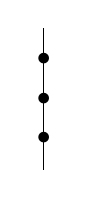
\begin{tikzpicture}[yscale=0.5,xscale=0.5]
\node at (0,1) {$\bullet$};
\node at (0,2) {$\bullet$};
\node at (0,3) {$\bullet$};
\draw (0,0.2) -- (0,3.8);
\end{tikzpicture}}}, 
\vcenter{\hbox{
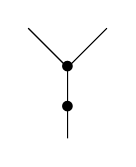
\begin{tikzpicture}[yscale=0.5,xscale=0.5]
\node at (0,1) {$\bullet$};
\node at (0,2) {$\bullet$};
\draw (0,0.2) -- (0,2) -- (1,3) ;
\draw (0,2) -- (-1, 3);
\end{tikzpicture}}}, 
\vcenter{\hbox{
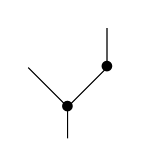
\begin{tikzpicture}[yscale=0.5,xscale=0.5]
\node at (0,1) {$\bullet$};
\node at (1,2) {$\bullet$};
\draw (0,0.2) -- (0,1) -- (1,2)--(1,3) ;
\draw (0,1) -- (-1, 2);
\end{tikzpicture}}}, 
\vcenter{\hbox{
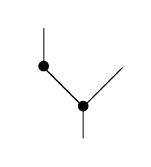
\begin{tikzpicture}[yscale=0.5,xscale=0.5]
\node at (0,1) {$\bullet$};
\node at (-1,2) {$\bullet$};
\draw (0,0.2) -- (0,1) -- (-1,2)--(-1,3) ;
\draw (0,1) -- (1, 2);
\end{tikzpicture}}}, 
\vcenter{\hbox{
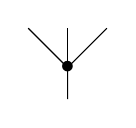
\begin{tikzpicture}[yscale=0.5,xscale=0.5]
\node at (0,1) {$\bullet$};
\draw (0,0.2) -- (0,1) -- (-1,2) ;
\draw (0,1) -- (1, 2);
\draw (0,1) -- (0, 2);
\end{tikzpicture}}}
\right\}\ .\]
\end{example}  

To any tree $\tau \in \mathrm{PT}^{[n]}$, we associate the element $\PP_\tau(p_0, \ldots, p_0)\in \F_n$ obtained by labelling the vertices of arity $k$ with $\PP_k$, the leaves with $p_0$, and by considering the global evaluation. 

\begin{example}
The planar tree 
\[\tau:=\vcenter{\hbox{
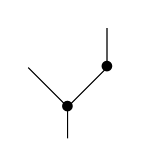
\begin{tikzpicture}[yscale=0.5,xscale=0.5]
\node at (0,1) {$\bullet$};
\node at (1,2) {$\bullet$};
\draw (0,0.2) -- (0,1) -- (1,2)--(1,3) ;
\draw (0,1) -- (-1, 2);
\end{tikzpicture}}}
\]
produces the element $\PP_\tau(p_0, \ldots, p_0)=\PP_2(p_0, \PP_1(p_0))\in \F_4$\ .
\end{example}


\begin{proposition}\label{prop:FixPtEqua}
The fixed-point equation 
\begin{eqnarray}\label{eqn:FixPt}
x=\PP(x)=p_0+\sum_{n=1}^{\infty}\PP_n\left(x^{\otimes n}\right)\ .
\end{eqnarray}
associated to any analytic function admits the following  unique solution:
\[
x=\sum_{n=1}^\infty \sum_{\tau \in \mathrm{PT}^{[n]}} \PP_\tau(p_0, \ldots, p_0)\ .
\]
\end{proposition}

\begin{proof}
Suppose that there exists a solution and let us write it as a series  $x=\sum_{n=1}^\infty x_n$, with $x_n\in \F_n$. The projection of Equation~\eqref{eqn:FixPt} onto $V/\F_{n+1}$, for $n\geqslant 1$, gives 
\begin{equation}\label{eqn:partial}
x_1+\cdots+x_{n}=p_0+\PP_1(x_1+\cdots+x_{n-1})+\cdots+\PP_{n-1}(x_1, \ldots, x_1)\ .\tag{*}
\end{equation}
By induction on $n\geqslant 1$, this shows that the  projection of $x$ onto $V/\F_{n+1}$ is unique, which proves that $x$ is unique since $(V, \F)$ is complete. 
In the other way round, let us consider 
\[
x_n:=\sum_{\tau \in \mathrm{PT}^{[n]}} \PP_\tau(p_0, \ldots, p_0) \in \F_n \qquad \text{and}
\qquad x:=\sum_{n=1}^\infty x_n\ .
\]
We now prove, by induction on $n\geqslant 1$, that $x$ satisfies the projection \eqref{eqn:partial} of  Equation~\eqref{eqn:FixPt} onto $V/\F_{n+1}$. 
For $n=1$, the set $\mathrm{PT}^{[0]}$ is made up of the trivial tree $|$, so $x_1=p_0$. Suppose now that the result holds true for $n$, and let us prove it for $n+1$:
\begin{eqnarray*}
p_0+\PP_1(x_1+\cdots+x_{n})+\cdots+\PP_{n}(x_1, \ldots, x_1)&=&p_0+\PP_1(x_1+\cdots+x_{n-1})+\cdots+\PP_{n-1}(x_1, \ldots, x_1)\\
&&+\PP_1(x_n)+\PP_2(x_1, x_{n-1})+\cdots+\PP_2(x_{n-1}, x_1)+\cdots\\
&&+\PP_{n+1}(x_1, \ldots, x_1) \\
&=&x_1+\cdots+x_{n} + \sum_{\tau \in \mathrm{PT}^{[n+1]}} \PP_\tau(p_0, \ldots, p_0)\\
&=&x_1+\cdots+x_{n+1}\ .
\end{eqnarray*}
\end{proof}

\subsection{Formal differential equations}

\bibliographystyle{alpha}
\bibliography{bib}

\medskip
\hrule\medskip
\bruno{\sc To do list:}
\begin{itemize}


\item \bruno{Applications : comparer avec ces notions d'\'equivalences des $\infty$-morphismes. Liens avec Dotsenko--Poncin}
\item \bruno{Etendre au cas a courbure [Bruno]}
\item Comprendre BCH (sup\'erieur) 
\item Holonomie ???
\item Quillen equivalence ? 
\item Lien avec Henriques 
\end{itemize}


\end{document}